\documentclass[10pt]{article}
\usepackage[utf8]{inputenc}
\usepackage[T1]{fontenc}
\usepackage{lmodern}
\usepackage[margin=0.85in,columnsep=0.32in]{geometry}
\usepackage{tikz}
\usetikzlibrary{arrows.meta,positioning,shapes.geometric}
\usepackage{booktabs}
\usepackage{xcolor}
\usepackage[hidelinks]{hyperref}
\usepackage{float}

\setlength{\parindent}{0pt}
\setlength{\parskip}{0.55em}

\definecolor{boxgreen}{RGB}{224,242,224}
\definecolor{boxyellow}{RGB}{252,244,214}
\definecolor{boxred}{RGB}{250,222,222}
\definecolor{boxgray}{RGB}{238,238,235}
\definecolor{lineblack}{RGB}{20,20,20}
\definecolor{barsolid}{RGB}{25,25,25}
\definecolor{bargray}{RGB}{143,143,137}

\title{\LARGE\bfseries El precipicio de herramientas:\\[2pt] El colapso categórico de un modelo pequeño donde los modelos grandes solo degradan}
\author{
  {\large Ricardo Martínez}\\[2pt]
  {\small Cloud Security \& Applied AI}
}
\date{\small Noviembre 2026}

\begin{document}
\twocolumn[
  \begin{@twocolumnfalse}
    \maketitle
    \begin{abstract}
    \noindent
    Un modelo de pesos abiertos de 9.7B, con una sola herramienta sintética, la llamó correctamente cada vez y completó un ciclo completo de reinyección de resultado. El mismo modelo, mismo backend, mismos parámetros de muestreo, conectado al catálogo de herramientas de producción de un agente real (más de veinte herramientas), nunca volvió a intentar una llamada real a lo largo de múltiples turnos en dos superficies independientes --- escribió el comando de shell como prosa en vez de invocarlo. Bajar la temperatura de muestreo arregló por completo el caso aislado y dejó intacto el caso de producción. Los benchmarks públicos ya documentan degradación por conteo de herramientas en modelos medianos y de frontera como una caída gradual de precisión; lo que este caso de campo aporta es la versión de un modelo pequeño del mismo eje, que se parece menos a una caída y más a una función escalón. La consecuencia práctica: certificar el tool-calling de un modelo con un solo conteo de herramientas no dice nada confiable sobre otro conteo, y la brecha no siempre es una pendiente.
    \end{abstract}
    \vspace{1.2em}
  \end{@twocolumnfalse}
]

\section{Dos mediciones del mismo modelo}

La primera prueba es con la que casi cualquier agente empieza: dale al modelo una herramienta, una instrucción clara de usarla, y confirma que lo hace. Un modelo de pesos abiertos de 9.7B pasó esto limpio --- una llamada a herramienta correctamente tipada, cada vez, seguida de un ciclo limpio de reinyección de resultado. Según esa prueba, el modelo es capaz de tool-calling.

La segunda prueba usó el mismo modelo exacto, el mismo backend exacto, los mismos parámetros de muestreo, conectado al catálogo real de herramientas desplegado en producción de una plataforma de agente personal: acceso a terminal, operaciones de archivo, búsqueda web, visión, generación de imágenes, voz, automatización de navegador, carga de habilidades, tareas programadas y mensajería, compuestas en catálogos que superan las veinte herramientas individuales. En dos superficies de entrada independientes --- un gateway de chat y una invocación directa por línea de comandos --- el modelo respondió en texto plano absolutamente todas las veces. Los logs propios de ambas superficies mostraron \texttt{api\_calls=1}: el modelo nunca llegó siquiera al turno de llamada a herramienta que requiere una invocación real. Narró un comando de shell como prosa en vez de llamar la herramienta de terminal que estaba justo ahí, en su payload.

\begin{table}[H]
\centering
\small
\begin{tabular}{@{}lll@{}}
\toprule
& \textbf{Prueba aislada} & \textbf{Prueba de producción} \\
\midrule
Herramientas ofrecidas & 1 (sintética) & 20+ (catálogo real) \\
Llamada intentada & Sí, cada turno & No, cero turnos \\
\texttt{api\_calls} & 2+ (ciclo real) & 1 (solo texto) \\
Superficies probadas & 1 & 2, independientes \\
\bottomrule
\end{tabular}
\caption{Mismo modelo, mismo backend, mismos parámetros de muestreo. La única variable que cambió entre columnas es cuántas herramientas había en el payload.}
\end{table}

\section{La hipótesis de la temperatura, a medias}

Los parámetros de muestreo por defecto del despliegue --- temperatura 1.0, penalización de presencia 1.5 --- parecían el sospechoso obvio. Esos valores favorecen continuaciones novedosas y de alta entropía, casi lo opuesto a lo que necesita un tool-calling determinista: un modelo que reproduzca confiablemente la llamada estructurada exacta que pide el esquema, no una original.

Se construyó y probó directamente contra la API del modelo una variante del mismo modelo con temperatura baja (0.1) y penalización de presencia en cero. Arregló por completo el caso aislado: una llamada a herramienta correctamente tipada, verificada de punta a punta con un ciclo completo de reinyección de resultado, sin ambigüedad de si fue casualidad. Conectado al mismo catálogo de producción bajo la misma variante de temperatura baja, en las mismas dos superficies independientes, el modelo siguió sin intentar una sola llamada a herramienta.

La hipótesis no estaba equivocada. Estaba incompleta. Los parámetros de muestreo importaron muchísimo para el caso de una herramienta y no explicaron nada del caso de producción. Lo que sea que bloquea el tool-calling una vez que el catálogo crece más allá de cierto umbral, no es principalmente un problema de muestreo para este modelo.

\section{Lo que ya muestra la literatura pública}

La degradación por conteo de herramientas en agentes LLM es un fenómeno documentado, reportado de forma desigual entre tamaños de modelo y diseños de benchmark:

\begin{itemize}
\item El benchmark ReAct de LangChain encontró que la precisión se mantuvo para \texttt{o1} pero cayó fuerte para \texttt{o3-mini} y casi a cero para \texttt{GPT-4o} al pasar de aproximadamente siete dominios, según el análisis de StackOne sobre el techo de conteo de herramientas.
\item La evaluación de Maxim AI de cinco modelos sobre catálogos de GitHub y Notion encontró que reducir las herramientas disponibles de 48 a 25 mejoró la precisión de todos los modelos probados, incluyendo Claude Sonnet 4 (66.67\% a 73.33\%).
\item El reporte propio de Anthropic sobre su Tool Search Tool muestra a Claude Opus 4.5 pasando de 79.5\% a 88.1\% en un benchmark interno al descubrir herramientas bajo demanda en vez de declararlas todas por adelantado --- cifra del proveedor, en su propio benchmark.
\item TSCG (mayo de 2026) reporta restaurar a Phi-4 14B de 0\% a 84.4\% de precisión con 20 herramientas mediante compilación de esquemas: un modelo mediano topando contra una pared a un conteo de herramientas comparable al medido aquí para un modelo más pequeño.
\end{itemize}

Un análisis de practicante sobre este cuerpo de trabajo lo dice claro: ningún benchmark público publica limpiamente el eje de decaimiento por tamaño --- fijar el modelo, variar el conteo de herramientas, graficar la precisión. La mayoría de las comparaciones publicadas fijan el conteo de herramientas y varían el modelo, o fijan el modelo y comparan exactamente dos conteos de herramientas elegidos para sostener una afirmación de producto específica, no una curva.

\section{Cómo se ve un precipicio, no una pendiente}

Los benchmarks de arriba describen decaimiento: la precisión baja a medida que sube el conteo de herramientas, pero para modelos capaces de tool-calling en absoluto, rara vez llega a cero. El modelo de 9.7B medido aquí no decayó entre los dos puntos probados --- fue confiable en uno e hizo cero llamadas reales en el otro, bajo dos regímenes de muestreo y dos superficies independientes.

\begin{figure}[H]
\centering
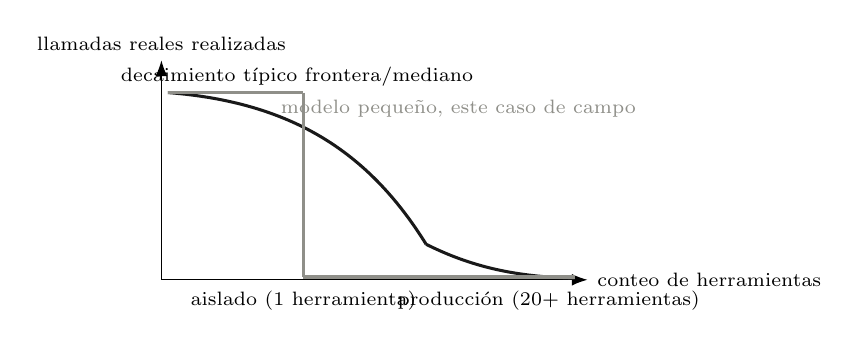
\begin{tikzpicture}[scale=0.82]
\draw[-{Latex[length=2mm]}, line width=0.5pt] (0,0) -- (6.6,0) node[right,font=\scriptsize] {conteo de herramientas};
\draw[-{Latex[length=2mm]}, line width=0.5pt] (0,0) -- (0,3.4) node[above,font=\scriptsize] {llamadas reales realizadas};
\draw[barsolid, line width=1.1pt] (0.1,2.9) .. controls (2.0,2.75) and (3.2,2.0) .. (4.1,0.55);
\draw[barsolid, line width=1.1pt] (4.1,0.55) .. controls (4.9,0.15) and (5.6,0.05) .. (6.4,0.02);
\node[font=\scriptsize] at (2.1,3.15) {decaimiento típico frontera/mediano};
\draw[bargray, line width=1.4pt] (0.1,2.9) -- (2.2,2.9);
\draw[bargray, line width=1.4pt] (2.2,2.9) -- (2.2,0.05);
\draw[bargray, line width=1.4pt] (2.2,0.05) -- (6.4,0.05);
\node[font=\scriptsize, text=bargray] at (4.6,2.65) {modelo pequeño, este caso de campo};
\node[font=\scriptsize] at (2.2,-0.32) {aislado (1 herramienta)};
\node[font=\scriptsize] at (6.0,-0.32) {producción (20+ herramientas)};
\end{tikzpicture}
\caption{Ilustrativo, no medido en un eje continuo: el patrón documentado de modelos de frontera/medianos es una caída a lo largo de la curva; los dos puntos medidos para el modelo pequeño en este caso son un escalón, no una pendiente.}
\end{figure}

Esta distinción importa para quien decide cuánto peso darle a una prueba de humo que pasó. Un decaimiento gradual se puede presupuestar --- enrutar las llamadas más difíciles a un modelo más grande, recortar el catálogo, aceptar una tasa de error conocida. Un paro categórico no se puede presupuestar igual: pasado el umbral que lo dispara, el modelo pequeño no está "algo menos confiable", no está participando en absoluto del contrato de tool-calling, en silencio, sin que se levante ningún error en ningún lado.

\section{Principio de diseño}

Certifica la capacidad de tool-calling de un modelo al conteo de herramientas con el que va a correr de verdad en producción, no al conteo que sea más barato de probar con una prueba de humo. Pasar con $N{=}1$ es evidencia sobre $N{=}1$. No es evidencia sobre $N{=}20$, y para un modelo pequeño, los dos pueden ser resultados categóricamente distintos en vez de puntos cercanos de una misma curva.

El patrón mínimo en \texttt{patterns/01\_isolated\_vs\_production\_toolset.py} vuelve esto concreto: una rutina de certificación que solo acepta a un modelo como capaz de usar herramientas si demuestra esa capacidad en el conteo real del despliegue, con tamaños de sondeo intermedios registrados para que un precipicio --- a diferencia de un decaimiento --- sea visible en cuanto aparece, no descubierto después en producción.

\section*{Nota metodológica}

Este es un caso de campo único, no un estudio controlado a través de múltiples modelos o catálogos de herramientas. Los dos conteos de herramientas, los parámetros de muestreo y las cifras de \texttt{api\_calls} citadas son mediciones reales del mismo sistema en dos superficies de entrada independientes, no simuladas. No se hace ninguna afirmación causal sobre el mecanismo --- dilución de atención, dilución de instrucciones por un system prompt más largo, o algo específico de esta familia de modelos --- solo que la prueba con conteo de herramientas aislado y la prueba con conteo de producción produjeron resultados categóricamente distintos para el mismo modelo bajo los mismos parámetros.

\begin{thebibliography}{9}
\bibitem{stackone} StackOne. \textit{The Agent Tool Count Ceiling}. stackone.com/blog/agent-tool-count-ceiling.
\bibitem{maxim} Maxim AI. \textit{Tool Chaos No More: How We're Measuring Model-Tool Accuracy in the Age of MCP}. getmaxim.ai/blog.
\bibitem{tscg} BenchmarkList. \textit{TSCG: Deterministic Tool-Schema Compilation for Agentic LLM Deployments}. benchmarklist.com.
\bibitem{hackernoon} HackerNoon. \textit{AI Agents Pick the Wrong Tool More Often as You Add Tools, and Research Shows Why}. hackernoon.com.
\end{thebibliography}

\end{document}
